 \let\negmedspace\undefined
\let\negthickspace\undefined
\documentclass[journal]{IEEEtran}
\usepackage[a5paper, margin=10mm, onecolumn]{geometry}
%\usepackage{lmodern} % Ensure lmodern is loaded for pdflatex
\usepackage{tfrupee} % Include tfrupee package

\setlength{\headheight}{1cm} % Set the height of the header box
\setlength{\headsep}{0mm}     % Set the distance between the header box and the top of the text
\usepackage{gvv-book}
\usepackage{gvv}
\usepackage{cite}
\usepackage{amsmath,amssymb,amsfonts,amsthm}
\usepackage{algorithmic}
\usepackage{graphicx}
\usepackage{textcomp}
\usepackage{xcolor}
\usepackage{txfonts}
\usepackage{listings}
\usepackage{enumitem}
\usepackage{mathtools}
\usepackage{gensymb}
\usepackage{comment}
\usepackage[breaklinks=true]{hyperref}
\usepackage{tkz-euclide} 
\usepackage{listings}
% \usepackage{gvv}                                        
\def\inputGnumericTable{}                                 
\usepackage[latin1]{inputenc}                                
\usepackage{color}                                            
\usepackage{array}                                            
\usepackage{longtable}                                       
\usepackage{calc}                                             
\usepackage{multirow}                                         
\usepackage{hhline}                                           
\usepackage{ifthen}                                           
\usepackage{lscape}



\usepackage{amsmath,amssymb}
\usepackage{booktabs}
\usepackage{tikz}
\usetikzlibrary{arrows.meta,angles,quotes}





\begin{document}

\bibliographystyle{IEEEtran}
\vspace{3cm}

\title{5.3.17}
\author{AI25BTECH11023 - Pratik R}
% \maketitle
% \newpage
% \bigskip
{\let\newpage\relax\maketitle}

\renewcommand{\thefigure}{\theenumi}
\renewcommand{\thetable}{\theenumi}
\setlength{\intextsep}{10pt} % Space between text and floats


\numberwithin{equation}{enumi}
\numberwithin{figure}{enumi}
\renewcommand{\thetable}{\theenumi}


\section*{\textbf{Question}}
Solve the system of linear equations using the matrix method 
\begin{align}
    7x+2y=11 \\
    4x-7y=2
\end{align}

\subsection*{\textbf{Solution:}} 
Using augmented matrix
\begin{align}
   \myvec{7 & 2 &\vrule &11 \\
   4 & -7 &\vrule &2}
\end{align}
Reducing it to reduced echelon form
\begin{align}
    \myvec{7 & 2 &\vrule &11 \\
   4 & -7 &\vrule &2} \xleftrightarrow{R_2 = R_2- R_1\times \frac{4}{7}} \myvec{7 & 2 &\vrule &11 \\
   0 & -\frac{57}{7} &\vrule &-\frac{30}{7}}
\end{align}
\begin{align}
\xleftrightarrow{R_2=R_2\times \frac{14}{57}} \myvec{7 & 2 &\vrule &11 \\
   0 & -2 &\vrule &-\frac{60}{57}}
    \xleftrightarrow{R_1 = R_1+ R_2} \myvec{7 & 0 &\vrule &\frac{567}{57} \\
   0 & -2 &\vrule &-\frac{60}{57}} 
\end{align}
\begin{align}
    \xleftrightarrow{R_1 = R_1/7} \myvec{1 & 0 &\vrule &\frac{81}{57} \\
   0 & -2 &\vrule &-\frac{60}{57}} \xleftrightarrow{R_2 = R_2/-2} \myvec{1 & 0 &\vrule &\frac{81}{57} \\
   0 & 1 &\vrule &\frac{30}{57}} 
\end{align}
Hence 
\begin{align}
    \myvec{x \\y} = \frac{1}{57} \myvec{81\\30}
\end{align}
\newpage
\begin{figure}[H]
\centering
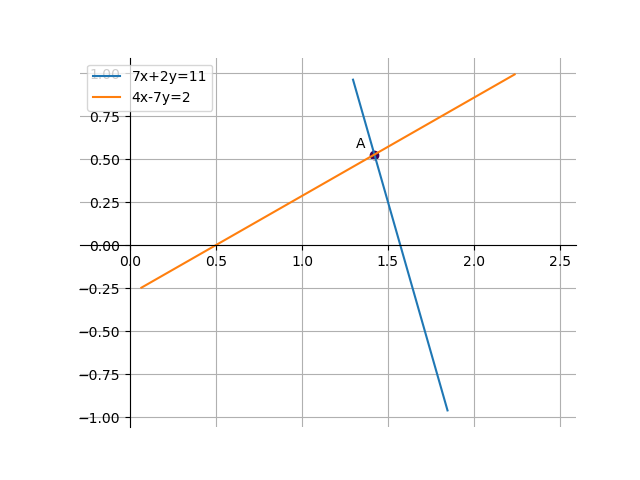
\includegraphics[width=0.7\columnwidth]{figs/fig.png} 
\caption{graph}
\label{}
\end{figure}

\end{document}
